\documentclass[a4paper,12pt]{article}

\usepackage[utf8]{inputenc}
\usepackage[T1]{fontenc}
\usepackage[polish]{babel}
\usepackage{amsmath, amssymb}
\usepackage{graphicx}
\usepackage{float}
\usepackage{hyperref}
\usepackage{geometry}
\usepackage{csvsimple} 

\usepackage{pgfplotstable}
\usepackage{booktabs}
\usepackage{siunitx} % do ładnego wyrównania liczb

\geometry{margin=2.5cm}

\sisetup{
    round-mode=places,
    round-precision=3,
    output-decimal-marker=.
}

\title{Sprawozdanie 2 z Statystyki i Modeli Liniowych}
\author{Wiktor Zoga}
\date{\today}

\begin{document}

\maketitle
\newpage

\section{Zadanie 1}

    Celem Zadania jest estymacje MLE dla $\mathbb{P}(X \ge 3)$ gdzie $X\sim Bin(m, p)$ ($ m = 5 $).

    Jako, że $ \mathbb{P}(X \ge 3) = \sum_{k=3}^{m} \binom{m}{k} p^k (1-p)^{m-k} $, 
    to estymator MLE dla $ \mathbb{P}(X \ge 3) $ jest dany przez:
    $$ \sum_{k=3}^{m} \binom{m}{k} \hat{p}_{MLE}^k (1-\hat{p}_{MLE})^{m-k} $$

    Aby obliczyć powyższy estymator, najpierw wyznaczyłem estymator MLE dla $p$:

    \begin{align*}
        L(p) &= \prod_{i=1}^{n} \binom{m}{x_i} p^{x_i} (1-p)^{m-x_i} \\
        \ell(p) &= \sum_{i=1}^{n} \left( \ln \binom{m}{x_i} + x_i \ln p + (m-x_i) \ln(1-p) \right) \\
        \frac{d\ell}{dp} &= \sum_{i=1}^{n} \left( \frac{x_i}{p} - \frac{m-x_i}{1-p} \right) \\     
    \end{align*}

    \begin{align*}
        \text{Z warunku } \frac{d\ell}{dp} = 0 &\Rightarrow \sum_{i=1}^{n} \left( \frac{x_i}{p} - \frac{m-x_i}{1-p} \right) = 0 \\
        &\Rightarrow \sum_{i=1}^{n} \left( x_i - m p \right) = 0 \\
        &\Rightarrow \hat{p}_{MLE} = \frac{\sum_{i=1}^{n} x_i}{n m}
    \end{align*}

    Druga pochodna to:
    \begin{align*}
        \frac{d^2\ell}{dp^2} &= \sum_{i=1}^{n} \left( -\frac{x_i}{p^2} - \frac{m-x_i}{(1-p)^2} \right) < 0
    \end{align*}
    co potwierdza, że znalezione rozwiązanie to maksimum lokalne, ale tez i globalne, ponieważ funkcja -log-wiarygodności jest wypukła.

    \subsection{Wyniki symulacji}

        \begin{center} 
            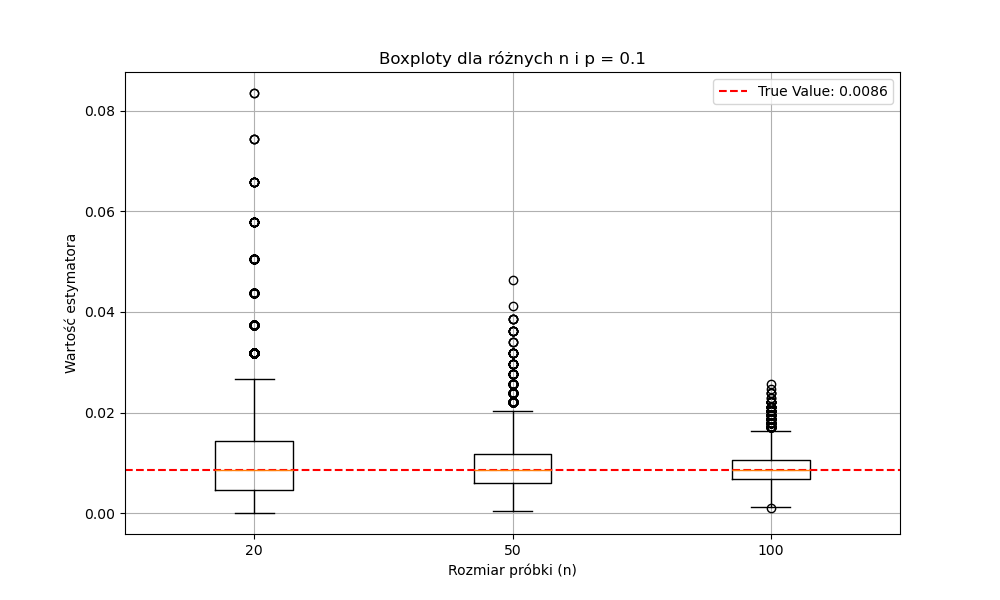
\includegraphics[width=0.9\textwidth]{../plots/zad1/boxploty/boxplot_p_1.png}
        \end{center}

        \begin{center} 
            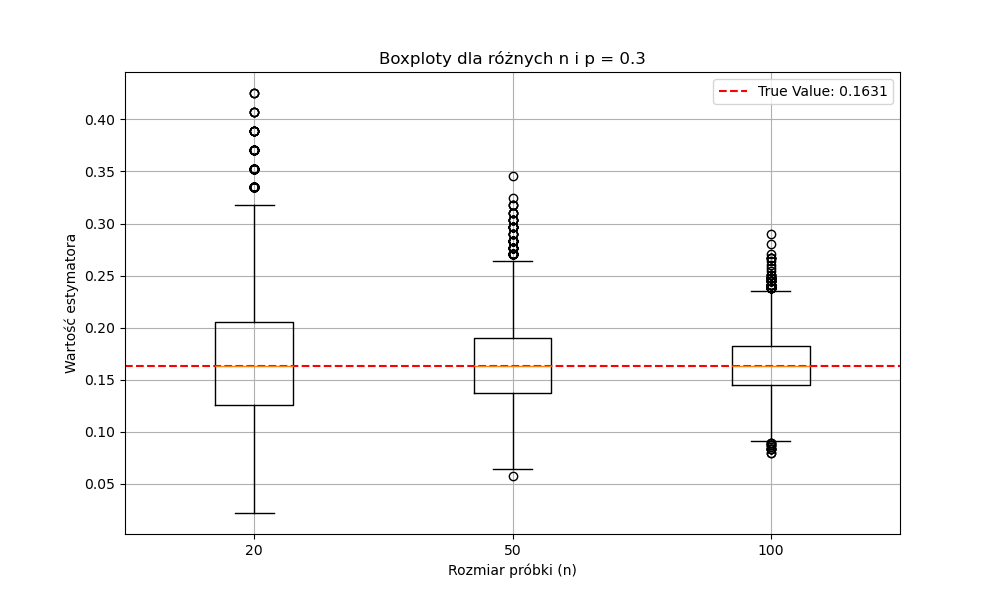
\includegraphics[width=0.9\textwidth]{../plots/zad1/boxploty/boxplot_p_3.png}
        \end{center}

        \begin{center} 
            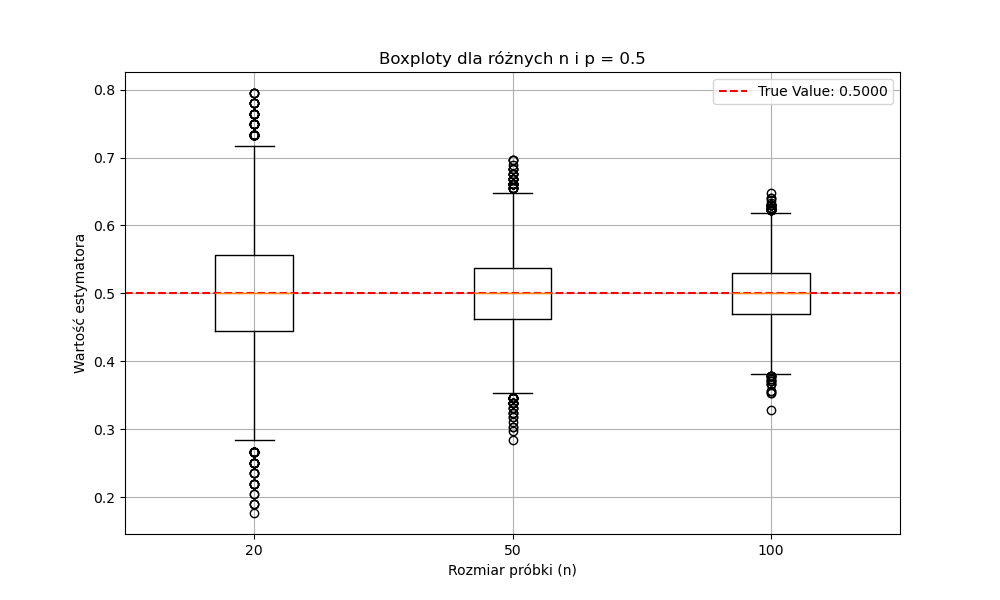
\includegraphics[width=0.9\textwidth]{../plots/zad1/boxploty/boxplot_p_5.png}
        \end{center}

        \begin{center} 
            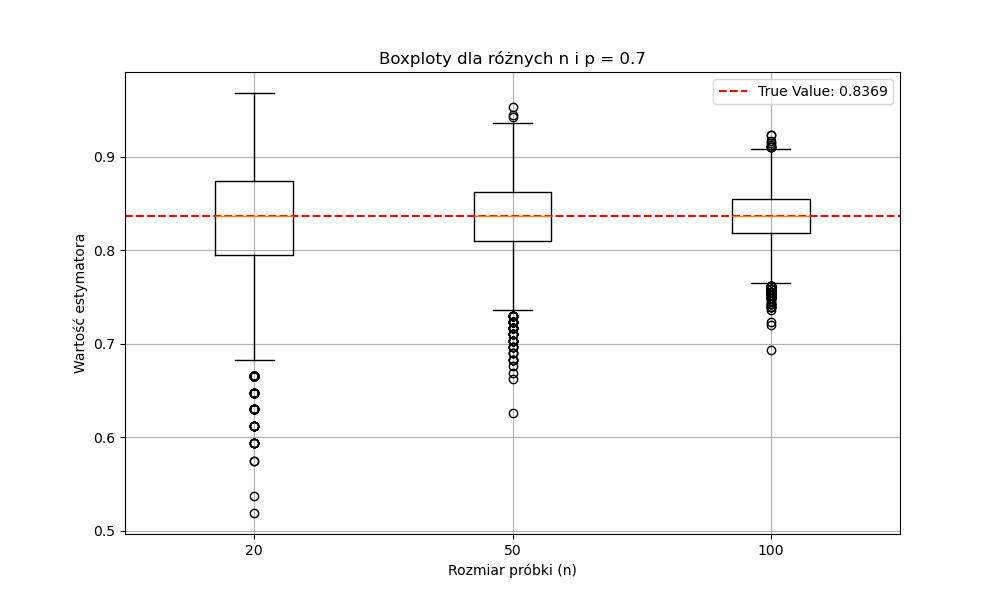
\includegraphics[width=0.9\textwidth]{../plots/zad1/boxploty/boxplot_p_7.png}
        \end{center}

        \begin{center} 
            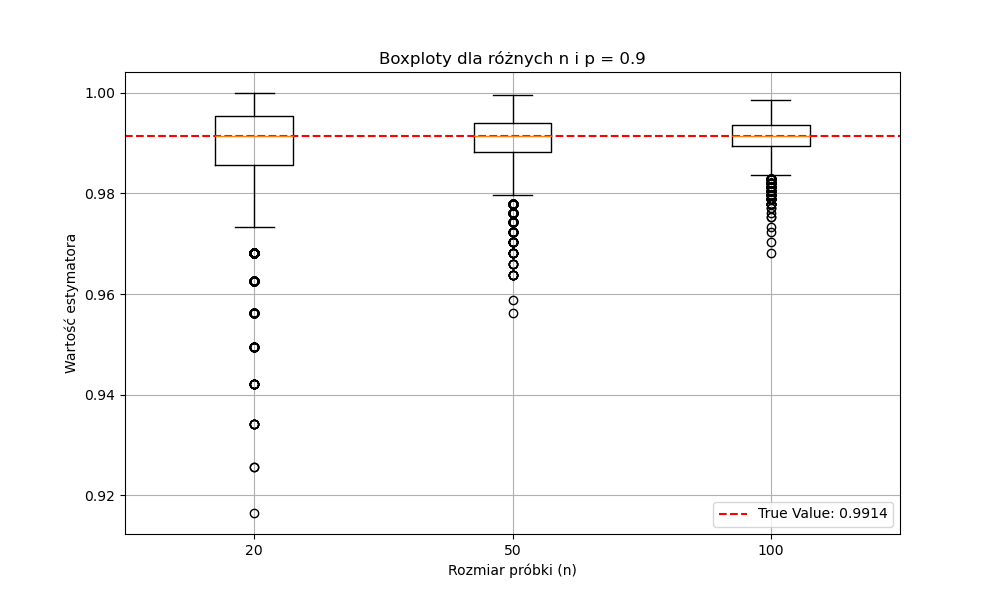
\includegraphics[width=0.9\textwidth]{../plots/zad1/boxploty/boxplot_p_9.png}
        \end{center}

        \begin{center} 
            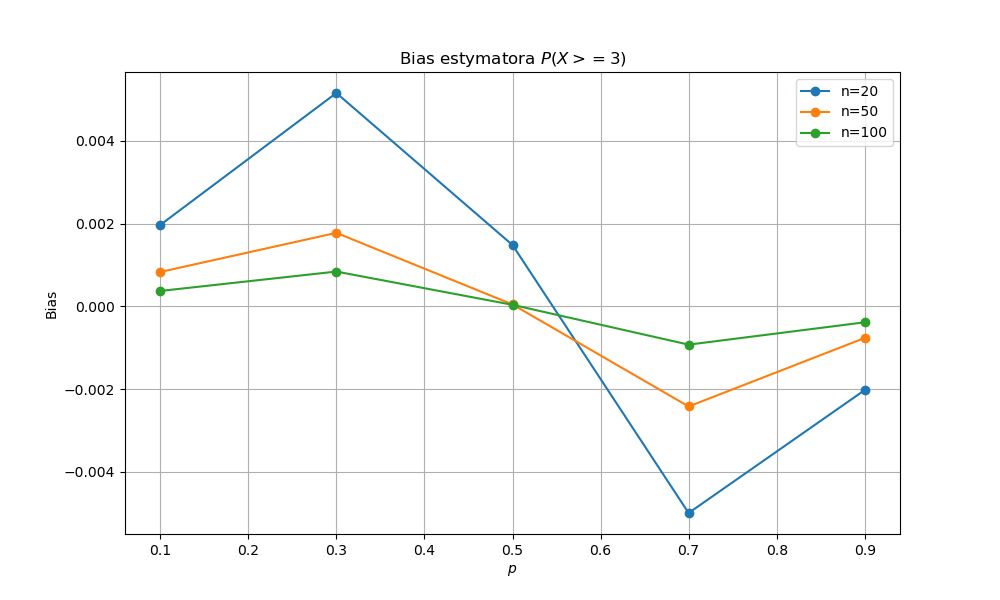
\includegraphics[width=0.9\textwidth]{../plots/zad1/wykresy_statystyk/bias_vs_p.png}
        \end{center}

        \begin{center} 
            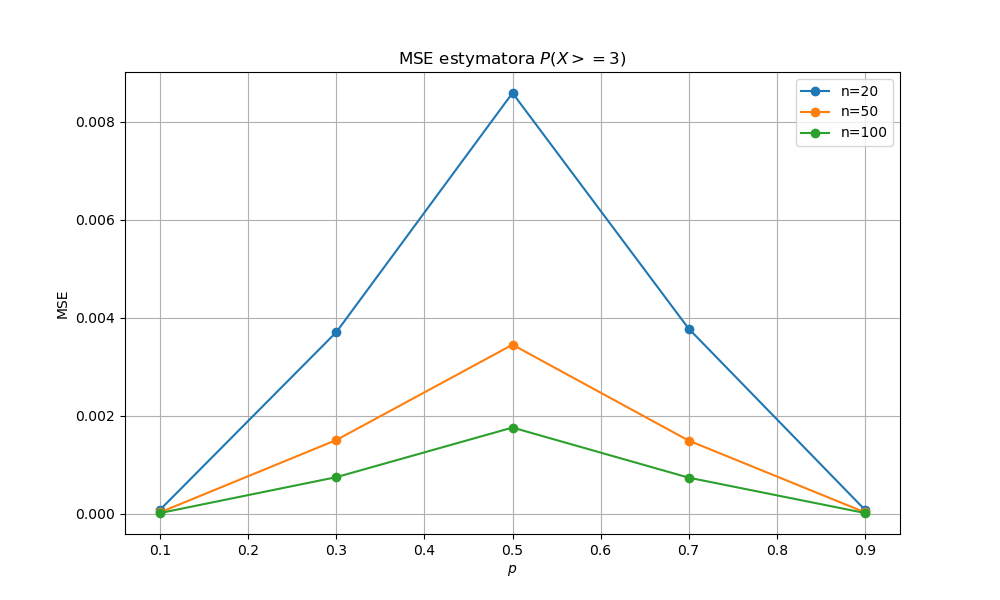
\includegraphics[width=0.9\textwidth]{../plots/zad1/wykresy_statystyk/mse_vs_p.png}
        \end{center}

        \begin{center} 
            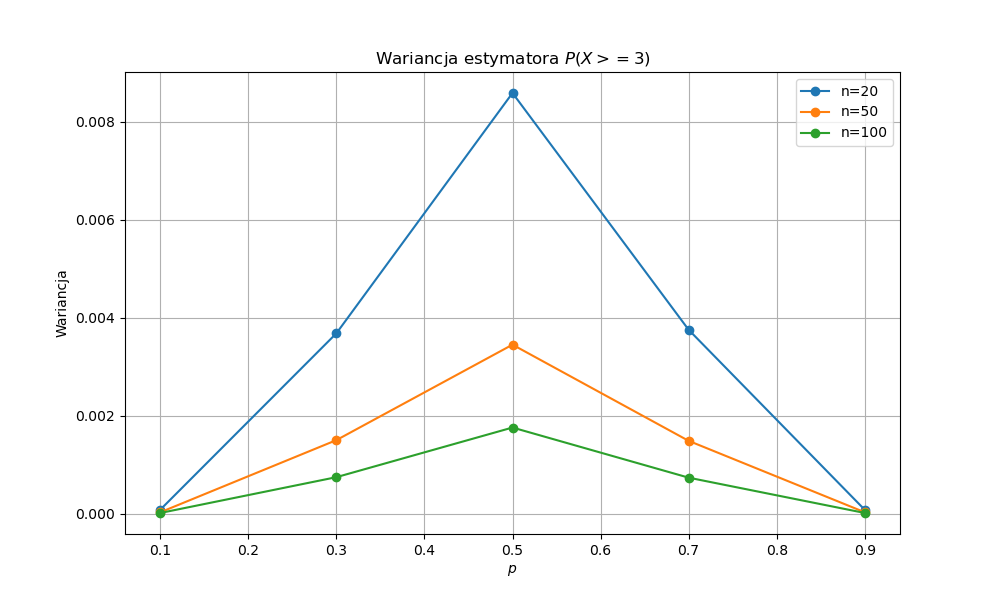
\includegraphics[width=0.9\textwidth]{../plots/zad1/wykresy_statystyk/variance_vs_p.png}
        \end{center}

    \subsection{Obserwacje z Boxplotów}
        \label{sec:boxploty}

        Wszystkie wykresy pudełkowe potwierdzają, że estymator jest asymptotycznie nieobciążony. Wraz ze wzrostem rozmiaru próby ($n = 20 \to 100$), rozrzut wyników (szerokość skrzynek i wąsów) znacząco maleje.

        \subsection{Analiza Metryk (Bias, Wariancja, MSE)}
        \label{sec:metryki}

        Analiza metryk w funkcji $p$ i $n$ ujawnia kluczowe zależności:

        \subsubsection*{Wpływ parametru $p$}
        \begin{itemize}
            \item Wariancja i MSE: Obydwie metryki osiągają maksymalną wartość w punkcie $p=0.5$ i maleją w kierunku krańcowych $p$ ($p=0.1, p=0.9$). Wynika to z faktu, że zmienność (wariancja) estymatora $\hat{p}$ jest proporcjonalna do $p(1-p)$, które jest największe dla $p=0.5$. Ten scenariusz charakteryzuje się największą niepewnością estymacji.
            \item Bias : Obciążenie jest generalnie niewielkie dla wszystkich scenariuszy, co świadczy o efektywności estymatora. Jest ono bliskie zeru w okolicach $p=0.5$.
        \end{itemize}

        \subsubsection*{Wpływ rozmiaru próby $n$}
        \begin{itemize}
            \item Redukcja Błędu: Najważniejszym trendem jest drastyczny spadek Wariancji i MSE wraz ze wzrostem $n$. Przejście z $n=20$ na $n=50$ przynosi największą poprawę precyzji.
            \item Bias: Obciążenie również zmniejsza się do zera wraz ze wzrostem $n$, co potwierdza asymptotyczną nieobciążoność.
        \end{itemize}

\newpage

\section{Zadanie 2}

    \subsection{Analiza Asymptotycznej Normalności $\hat{\theta}_{\text{MLE}}$ dla $\text{Beta}(\theta, 1)$}

    Przeprowadzono symulację w celu zbadania rozkładu estymatora $\hat{\theta}_{\text{MLE}}$ parametru $\theta$ 
    w rozkładzie $\text{Beta}(\theta, 1)$ oraz zweryfikowania jego zbieżności do rozkładu normalnego.
    Informację Fishera, $I(\theta)$, oszacowano empirycznie ($\hat{I}_n$) 
    i wykorzystano do określenia teoretycznej wariancji asymptotycznej $V_{\text{asymp}} = 1/\hat{I}_n$.

    \subsection{Wyniki symulacji dla $\theta$=$0.5$}

        \begin{center} 
            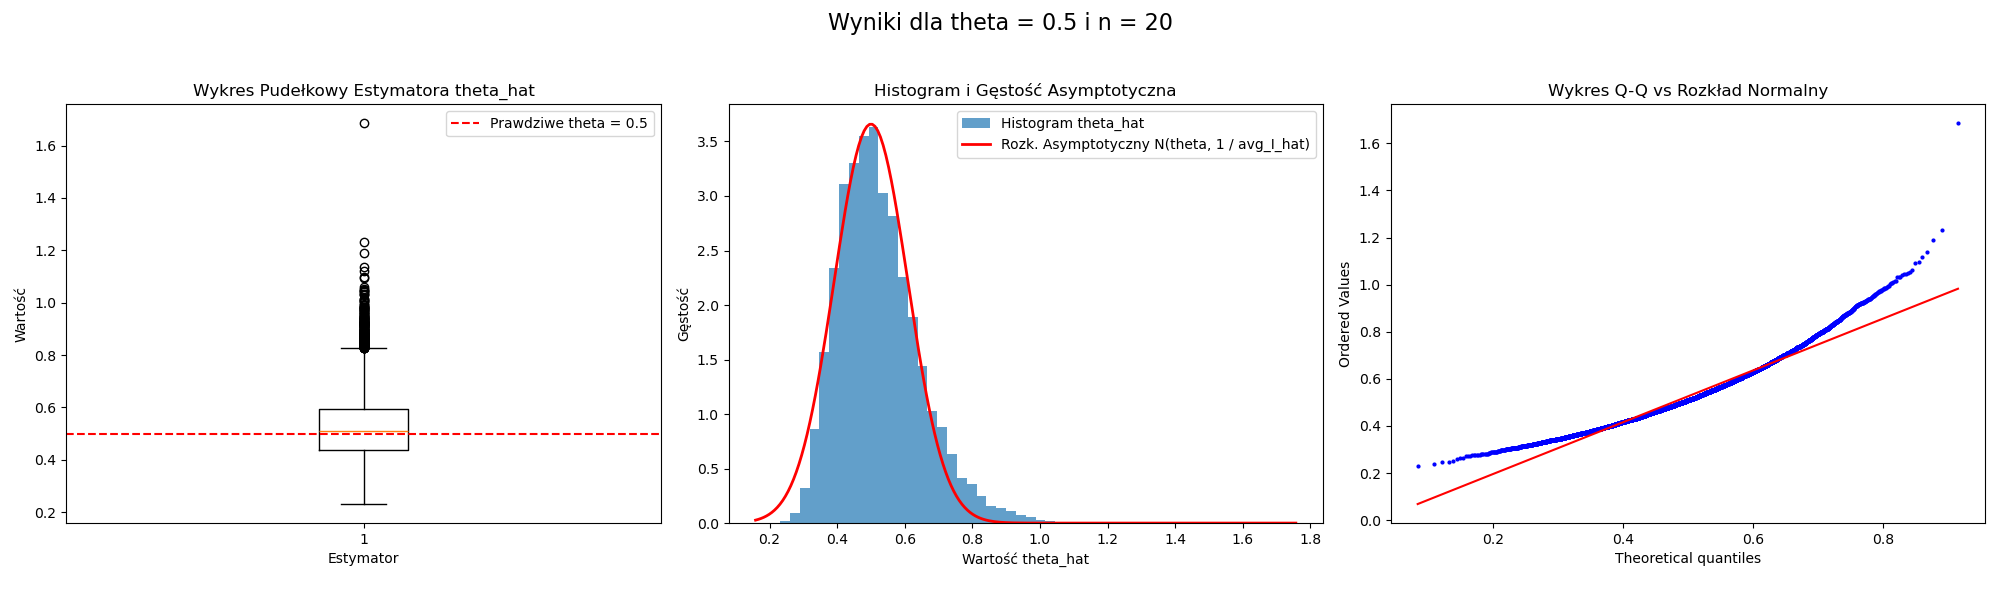
\includegraphics[width=0.9\textwidth]{../plots/zad2/wyniki_wykresy/results_theta_0.5_n_20.png}
        \end{center}

        \begin{center} 
            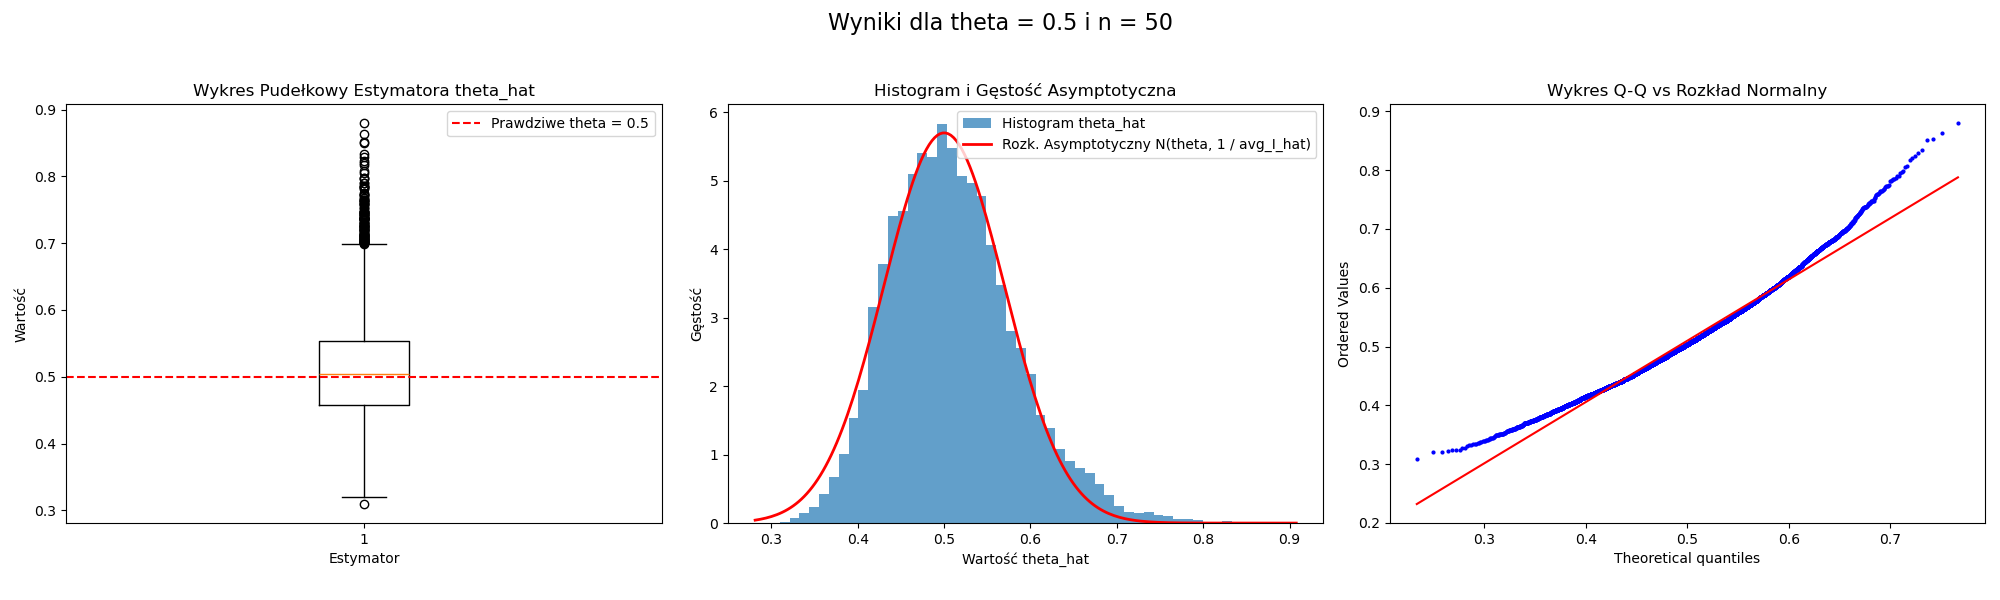
\includegraphics[width=0.9\textwidth]{../plots/zad2/wyniki_wykresy/results_theta_0.5_n_50.png}
        \end{center}

        \begin{center} 
            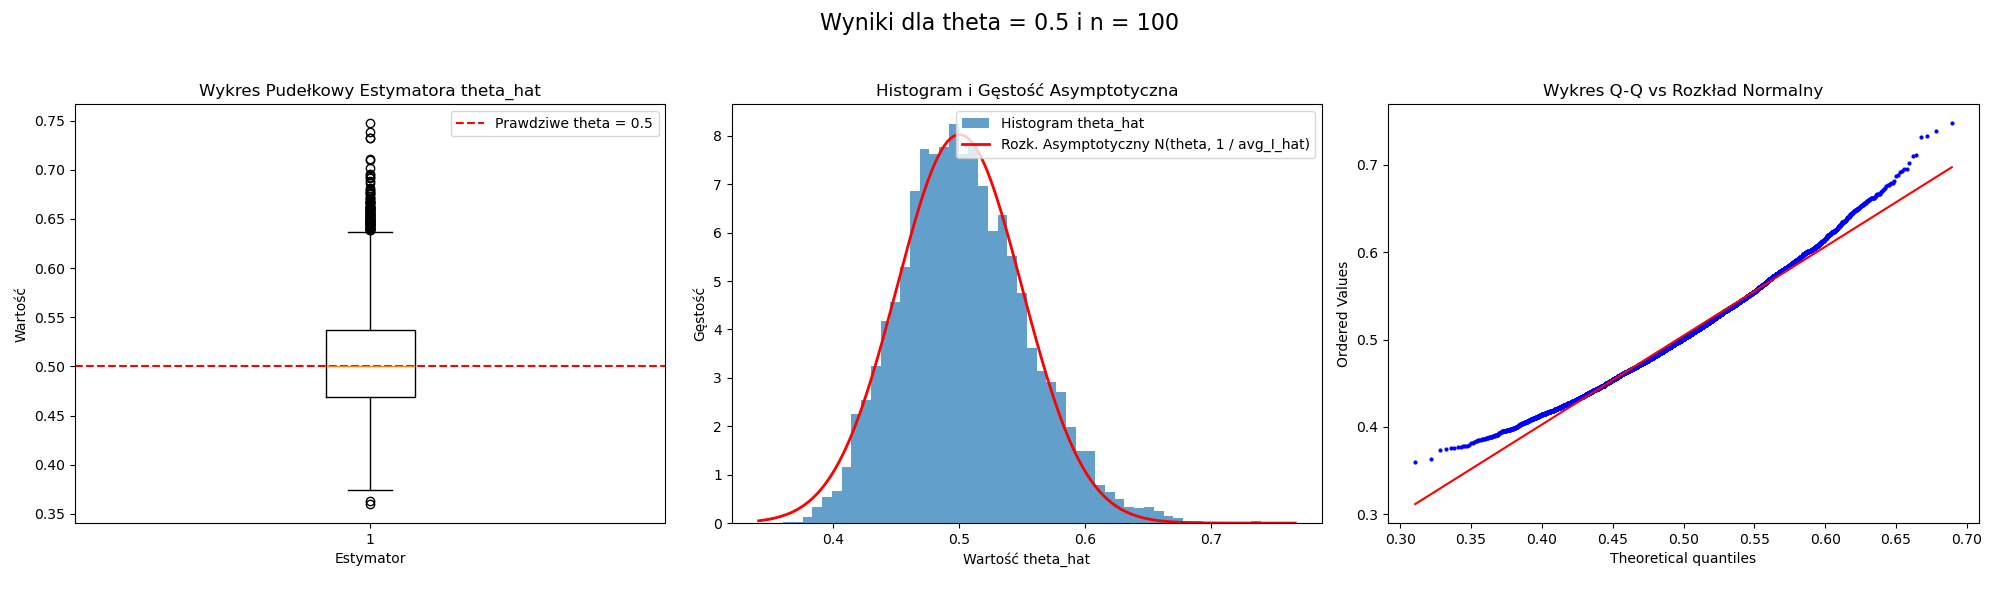
\includegraphics[width=0.9\textwidth]{../plots/zad2/wyniki_wykresy/results_theta_0.5_n_100.png}
        \end{center}
    \subsection{Wyniki symulacji dla $\theta$=$1$}

        \begin{center} 
            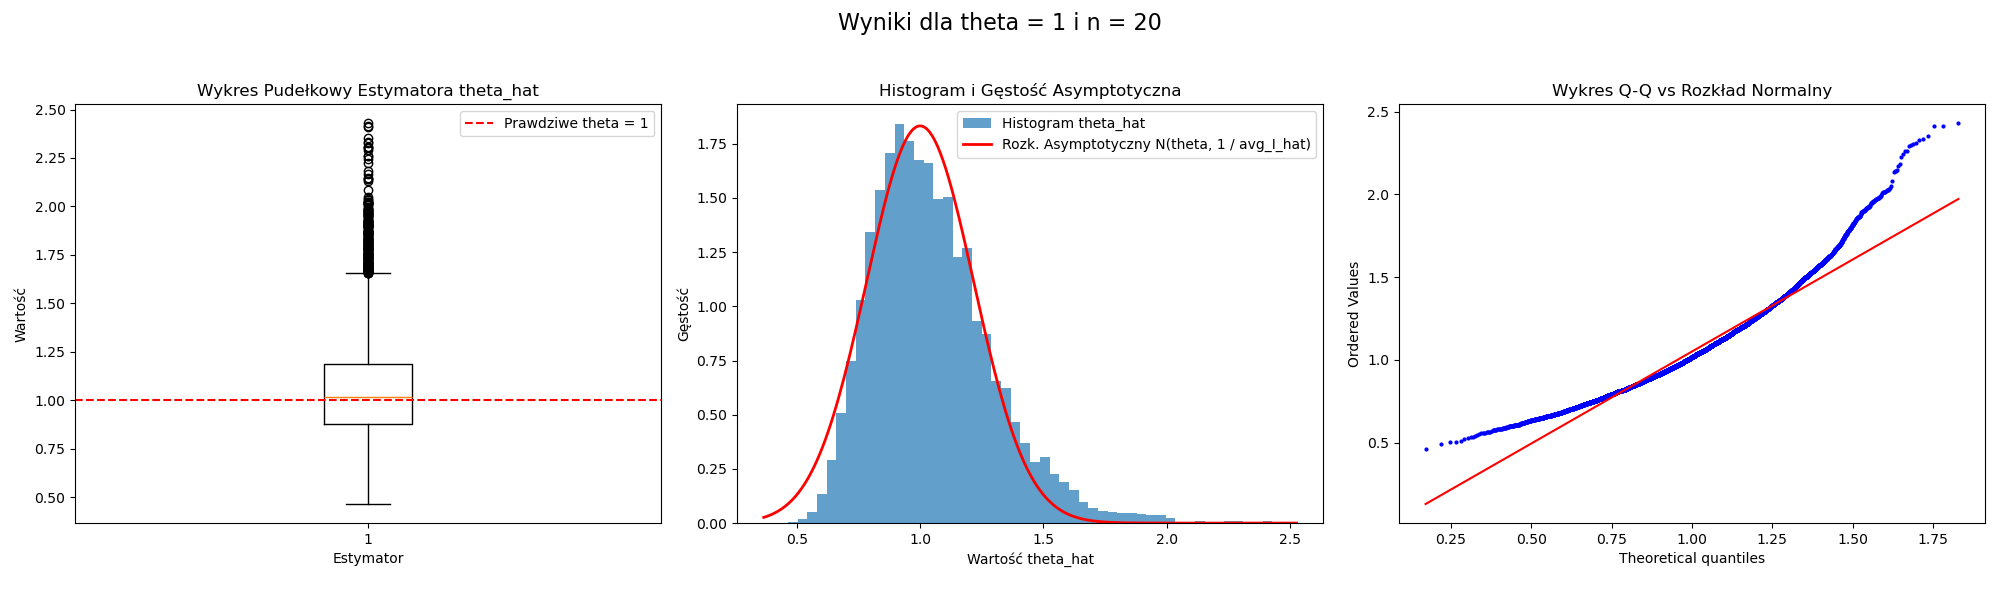
\includegraphics[width=0.9\textwidth]{../plots/zad2/wyniki_wykresy/results_theta_1_n_20.png}
        \end{center}

        \begin{center} 
            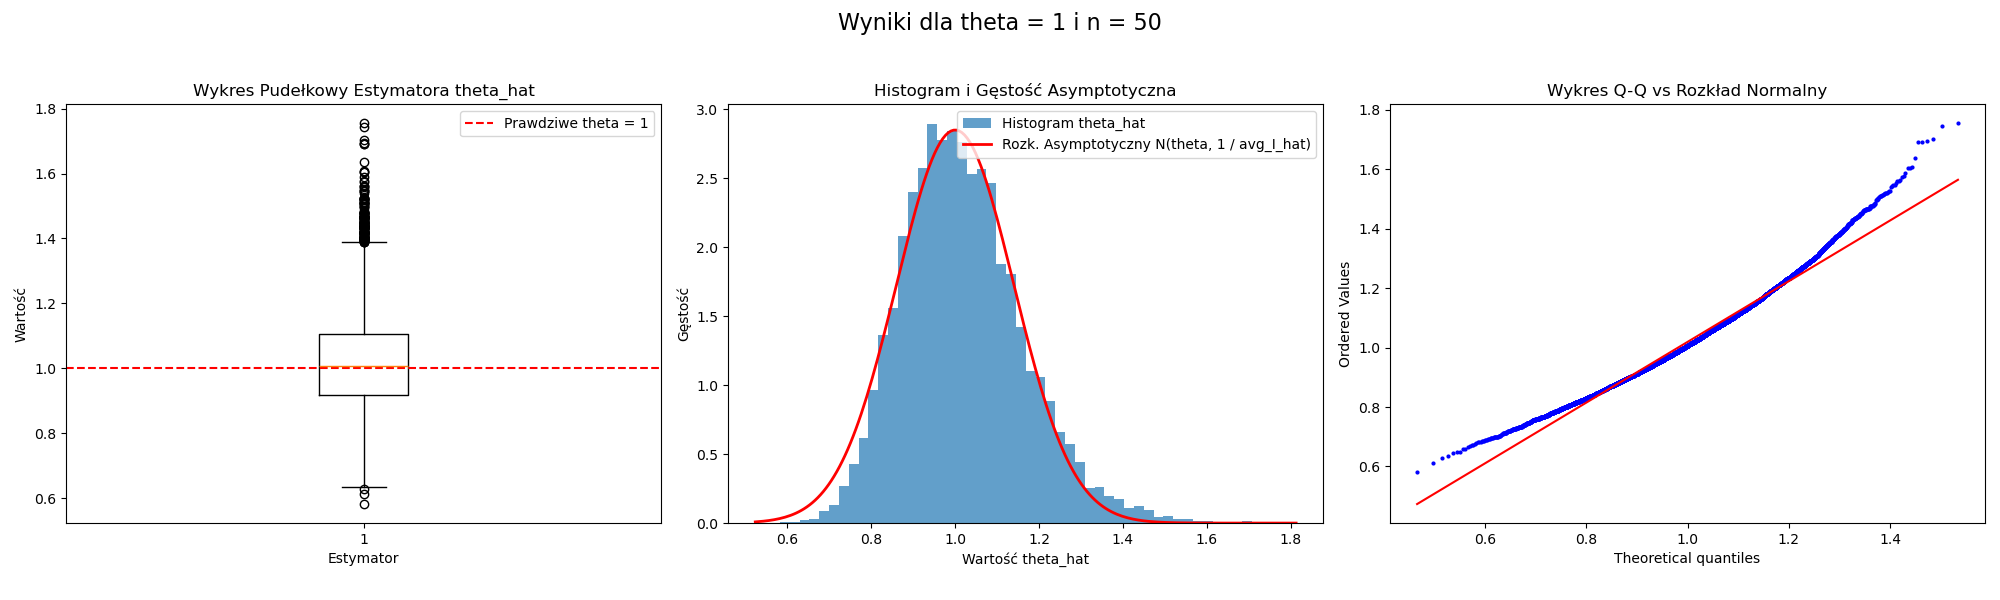
\includegraphics[width=0.9\textwidth]{../plots/zad2/wyniki_wykresy/results_theta_1_n_50.png}
        \end{center}

        \begin{center} 
            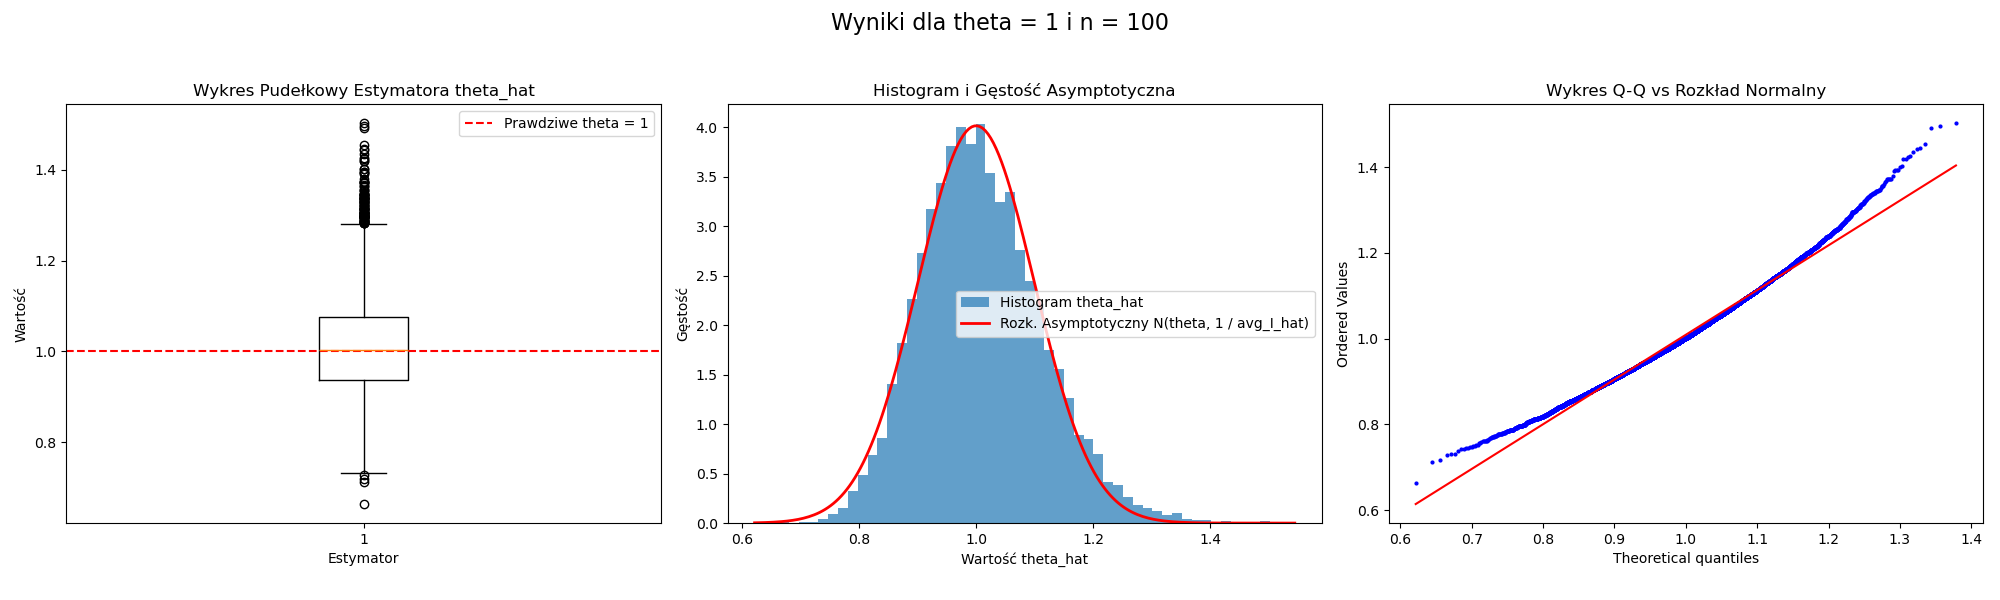
\includegraphics[width=0.9\textwidth]{../plots/zad2/wyniki_wykresy/results_theta_1_n_100.png}
        \end{center}
    \subsection{Wyniki symulacji dla $\theta$=$2$}

        \begin{center} 
            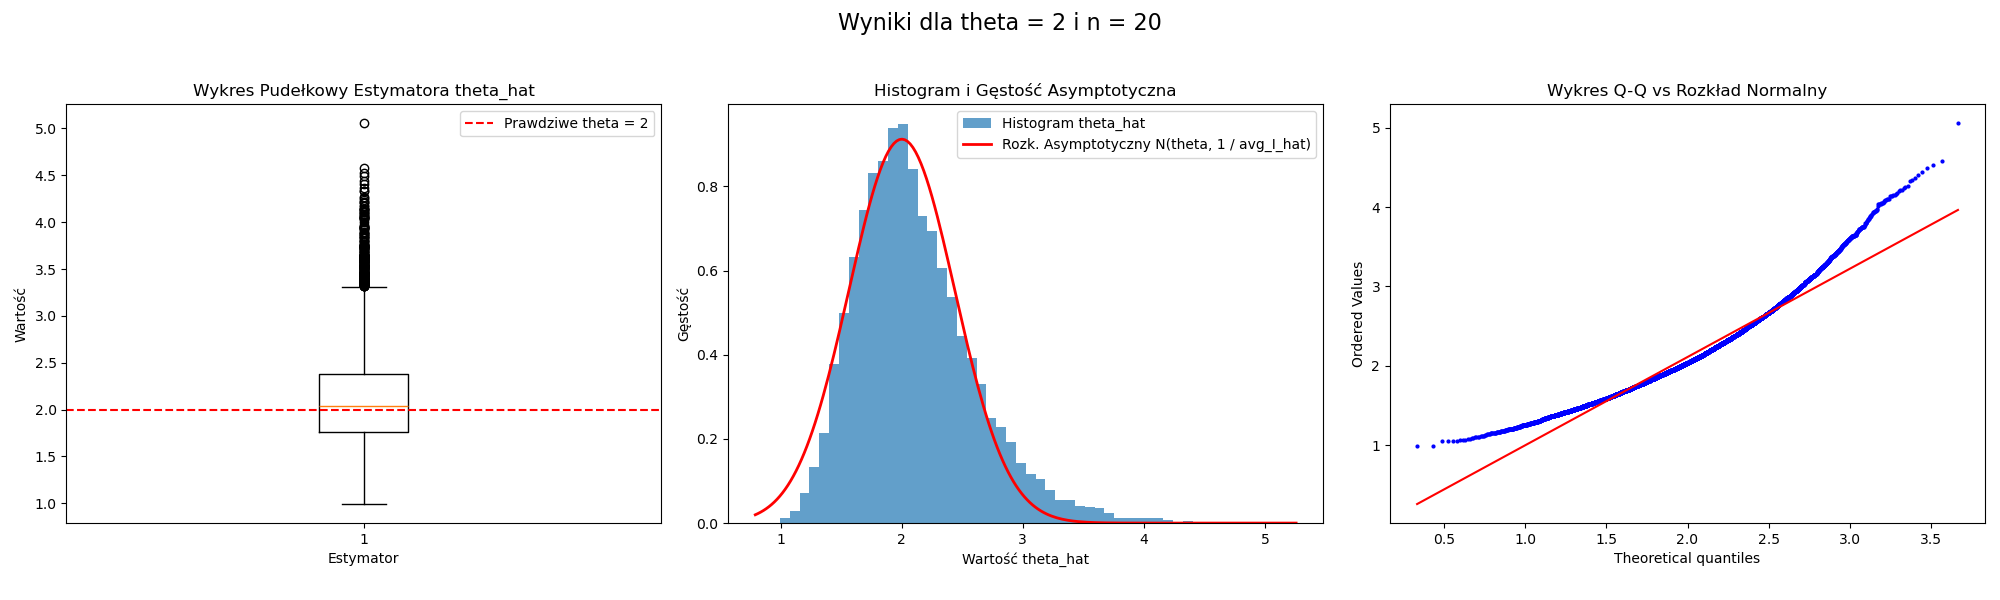
\includegraphics[width=0.9\textwidth]{../plots/zad2/wyniki_wykresy/results_theta_2_n_20.png}
        \end{center}

        \begin{center} 
            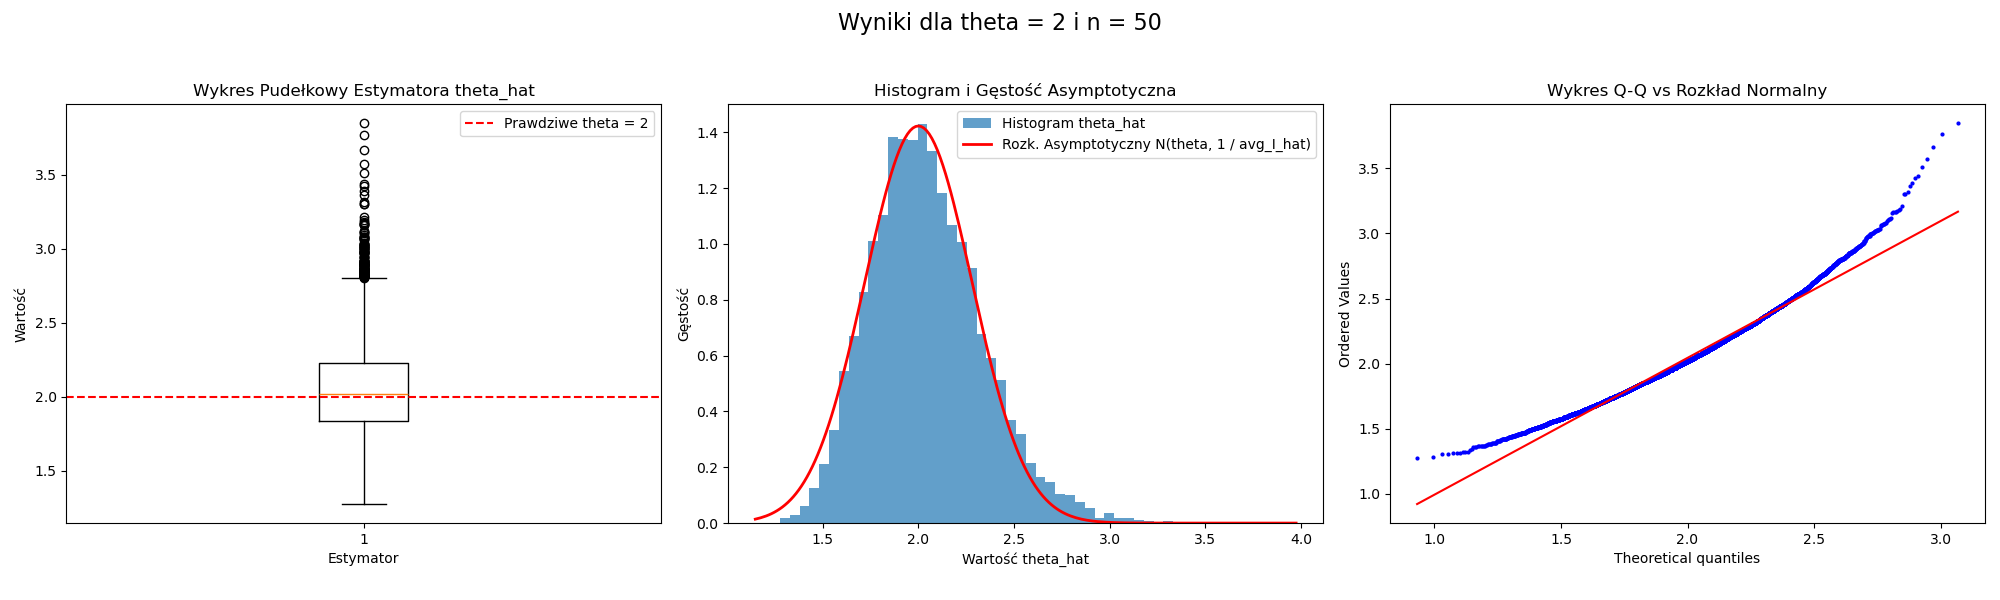
\includegraphics[width=0.9\textwidth]{../plots/zad2/wyniki_wykresy/results_theta_2_n_50.png}
        \end{center}
        
        \begin{center} 
            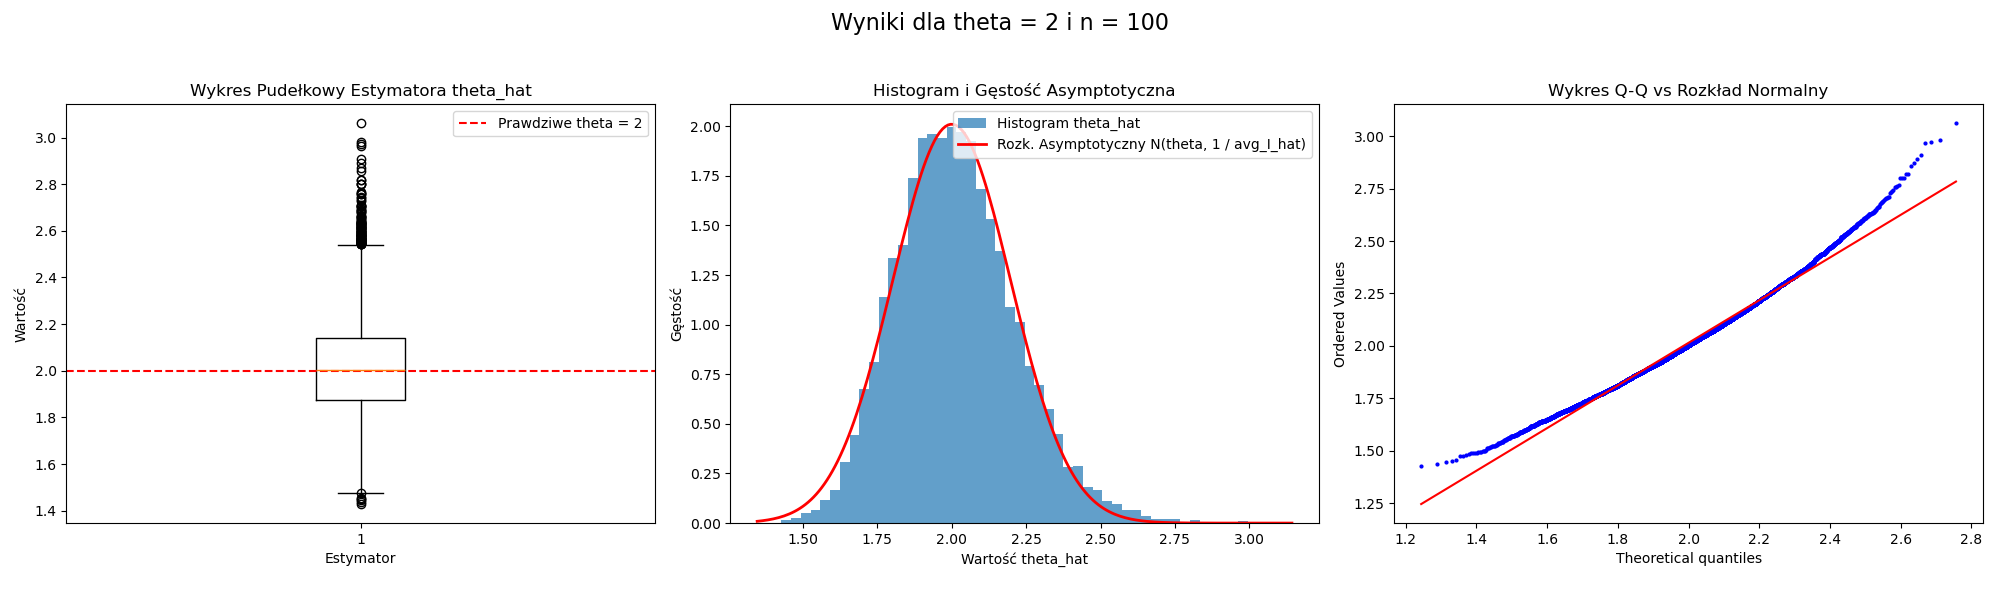
\includegraphics[width=0.9\textwidth]{../plots/zad2/wyniki_wykresy/results_theta_2_n_100.png}
        \end{center}


    \subsection{Wnioski na podstawie wykresów rozkładu}

        Wykresy dla poszczególnych scenariuszy ($\theta \in \{0.5, 1, 2, 5\}$, $n \in \{20, 50, 100\}$) dostarczają wizualnego potwierdzenia właściwości estymatora:

        \begin{itemize}
            \item \textbf{Boxploty:} Potwierdzają \textbf{asymptotyczną nieobciążoność} estymatora. 
            Mediana wyników jest w każdym przypadku zbieżna z prawdziwą wartością $\theta$.
            \item \textbf{Histogram i Gęstość Asymptotyczna:} Wraz ze wzrostem $n$, histogram wyników 
            $\hat{\theta}_{\text{MLE}}$ coraz ściślej \textbf{pokrywa się z krzywą gęstości rozkładu normalnego} $N(\theta, 1/\hat{I}_n)$. 
            Już dla $n=50$, a zwłaszcza dla $n=100$, dopasowanie jest bardzo dobre.
            \item \textbf{Wykres Kwantylowo-Kwantylowy:} Jest to \textbf{potwierdzenie normalności} rozkładu. 
            Punkty oszacowań układają się wzdłuż prostej, szczególnie dla $n=100$, co uzasadnia tezę o asymptotycznej normalności. 
            Odbieganie punktów na krańcach rozkładu dla $n=20$ sugeruje, że przy małej próbie zbieżność nie została jeszcze w pełni osiągnięta.
        \end{itemize}
    
    \subsection{Uzasadnienie Asymptotycznej Normalności}

        Rozkład $\hat{\theta}_{\text{MLE}}$ jest \textbf{asymptotycznie normalny}. Zgodnie z teorią:
        $$
        \sqrt{n}(\hat{\theta}_{\text{MLE}} - \theta) \xrightarrow{d} N\left(0, \frac{1}{I_1(\theta)}\right)
        $$
        gdzie $I_1(\theta)$ jest informacją Fishera dla pojedynczej obserwacji.
        Nasza symulacja empirycznie wspiera to twierdzenie,
        wykazując doskonałe dopasowanie rozkładu estymatora do rozkładu normalnego wraz ze wzrostem $n$.

    

        \newpage

    \subsection{Analiza Metryk (Wpływ $\theta$ i $n$)}

        Tabela statystyk dostarcza ilościowego porównania:

        \pgfplotstableread[col sep=comma]{../plots/zad2/podsumowanie_statystyk.csv}\datatable
        \begin{table}[h!]
            \centering
            \pgfplotstabletypeset[
                columns={theta_true,n,mean_theta_hat,bias,var_asymp_theo,var_asymp_est,var_simulacji},
                columns/theta_true/.style={column name={$\theta_{\text{true}}$}},
                columns/n/.style={column name={$n$}},
                columns/mean_theta_hat/.style={column name={$\hat{\theta}_{\text{mean}}$}},
                columns/bias/.style={column name={Bias}},
                columns/var_asymp_theo/.style={column name={Var$_{\text{teo}}$}},
                columns/var_asymp_est/.style={column name={Var$_{\text{est}}$}},
                columns/var_simulacji/.style={column name={Var$_{\text{sim}}$}},
                every head row/.style={before row=\toprule,after row=\midrule},
                every last row/.style={after row=\bottomrule}
            ]{\datatable}
        \end{table}

    
        \subsubsection*{Wpływ rozmiaru próby $n$}
            \begin{itemize}
                \item \textbf{Precyzja:} Wariancja \textbf{maleje} wraz ze wzrostem $n$. Estymator jest najbardziej precyzyjny dla $n=100$.
                \item \textbf{Zbieżność Wariancji:} Wraz ze wzrostem $n$, wariancja symulacji staje się coraz bardziej zbieżna z teoretyczną 
                \textbf{Wariancją Asymptotyczną} ($1/\hat{I}_n$), co dodatkowo potwierdza efektywność estymatora.
            \end{itemize}

        \subsubsection*{Wpływ parametru $\theta$}
            \begin{itemize}
                \item \textbf{Wariancja i MSE:} Wariancja oszacowania jest najmniejsza dla \textbf{największej wartości $\theta$} ($\theta=5$) i wzrasta dla mniejszych $\theta$. 
                Oznacza to, że estymacja $\theta$ jest najbardziej precyzyjna, gdy rozkład $\text{Beta}(\theta, 1)$ jest przesunięty w kierunku $x=1$.
                \item \textbf{Kształt Rozkładu:} Dla małych $\theta$ ($\theta=0.5$), 
                rozkład $\hat{\theta}_{\text{MLE}}$ jest często bardziej skośny i wymaga większego $n$ do osiągnięcia symetrii i pełnej normalności.
            \end{itemize}


\newpage

\section{Zadanie 3}
    
    W zadaniu zbadano właściwości estymatora $\hat{\theta}_{\text{MLE}}$ parametru lokalizacji $\theta$ w rozkładzie $\text{Logist}(\theta, \sigma)$, przy założeniu, że parametr skali $\sigma$ jest znany. Wykorzystano metodę Newtona-Raphsona do numerycznego wyznaczenia $\hat{\theta}_{\text{MLE}}$,
    badając scenariusze różniące się parametrami $(\theta, \sigma)$ oraz rozmiarem próby $n \in \{20, 50, 100\}$.

    \begin{center} 
        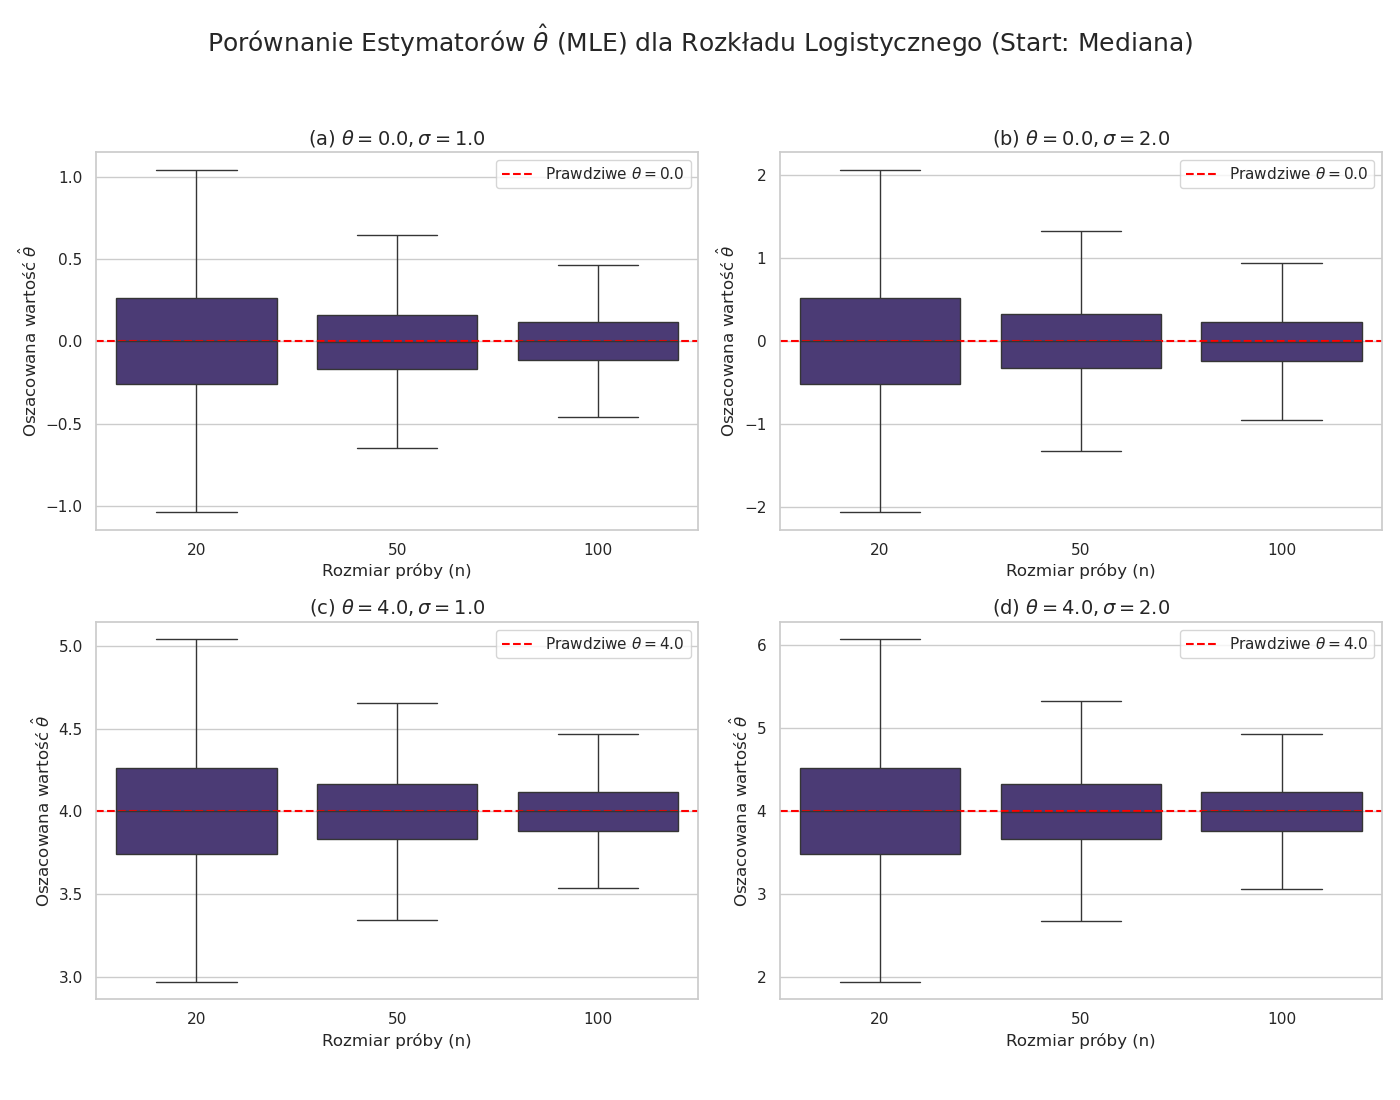
\includegraphics[width=0.9\textwidth]{../plots/zad3/wykresy_boxplot/mle_logistic_boxplot_comparison.png}
    \end{center}

    \pgfplotstableread[col sep=comma]{../plots/zad3/statystyki_metryki/podsumowanie_metryk_mle_logistic_MEDIANA.csv}\datatable

    \begin{table}[h!]
        \centering
        \pgfplotstabletypeset[
            columns={n,true_theta,true_sigma,Bias,Variance,MSE},
            columns/n/.style={column name={$n$}},
            columns/true_theta/.style={column name={$\theta$}},
            columns/true_sigma/.style={column name={$\sigma$}},
            columns/Bias/.style={column name={Bias}},
            columns/Variance/.style={column name={Variance}},
            columns/MSE/.style={column name={MSE}},
            every head row/.style={before row=\toprule,after row=\midrule},
            every last row/.style={after row=\bottomrule}
        ]{\datatable}
    \end{table}


    \subsection{Właściwości Estymatora (Boxploty i Metryki)}

    \subsubsection*{Ocena Metryk (Bias, Wariancja, MSE)}

    \begin{itemize}
        \item \textbf{Obciążenie (Bias):} We wszystkich scenariuszach Bias jest \textbf{bardzo bliski zeru}. Wartości obciążenia maleją wyraźnie wraz ze wzrostem $n$. To potwierdza, że estymator $\hat{\theta}_{\text{MLE}}$ jest \textbf{asymptotycznie nieobciążony}.
        \item \textbf{Wariancja i MSE:} Obie metryki maleją \textbf{proporcjonalnie do $1/n$}. Wzrost $n$ z $20$ do $100$ skutkuje radykalnym wzrostem precyzji (spadkiem wariancji). 
    \end{itemize}

    \subsubsection*{Wpływ parametru skali $\sigma$}
    Wykresy pokazują wyraźną zależność Wariancji i MSE od $\sigma$:
    \begin{itemize}
        \item \textbf{Większa skala, większy błąd:} Scenariusze z $\sigma = 2.0$  charakteryzują się \textbf{znacznie większym MSE i Wariancją} w porównaniu do scenariuszy z $\sigma = 1.0$, przy tym samym $n$.
        \item \textbf{Uzasadnienie:} Parametr $\sigma$ kontroluje rozrzut całego rozkładu. Większa wartość $\sigma$ oznacza większą zmienność danych, co bezpośrednio przekłada się na większą wariancję estymatora $\hat{\theta}_{\text{MLE}}$.
    \end{itemize}

    \subsection{Punkt Startowy}
    Wybranym punktem startowym dla algorytmu Newtona-Raphsona była mediana próby.
    W przyadku innch punktów startowych (np. średnia, maximum, stała) tempo zbieżności było różne. 
    Dlatego wybór punktu startowego ma istotne znaczenie dla efektywności algorytmu.

    \pgfplotstableread[col sep=comma]{../plots/zad3/statystyki_metryki/srednia_liczba_krokow.csv}\datatable

    \begin{table}[h!]
        \centering
        \begin{tabular}{l r}
            \toprule
            Strategia startowa & Średnia liczba iteracji \\
            \midrule
            Maksimum   & 37.551 \\
            Mediana    & 2.927  \\
            Stała 0.0  & 7.421  \\
            Średnia    & 2.856  \\
            \bottomrule
        \end{tabular}
        \caption{Średnia liczba kroków algorytmu dla różnych strategii startowych}
    \end{table}

\newpage

\section{Zadanie 4a}

    W zadaniu przeprowadzono symulację w celu porównania właściwości estymatora $\hat{\theta}_{\text{MLE}}$ oraz estymatora $\hat{\theta}_{\text{MOM}}$
    dla parametru $\theta$ w rozkładzie $\text{Beta}(\theta, 1)$.

    \subsection{Definicje Estymatorów}

        \begin{itemize}
            \item \textbf{Estymator Największej Wiarogodności:} Dla $\text{Beta}(\theta, 1)$ jest dany wzorem $\hat{\theta}_{\text{MLE}} = \frac{-1}{\sqrt{\overline(\ln(X))}}$.
            \item \textbf{Estymator Metody Momentów:} Wyznaczony z pierwszego momentu centralnego: $\hat{\theta}_{\text{MOM}} = \frac{\bar{X}}{1 - \bar{X}}$.
        \end{itemize}

    \subsection{Analiza Rozkładu Estymatorów}

        \begin{center} 
            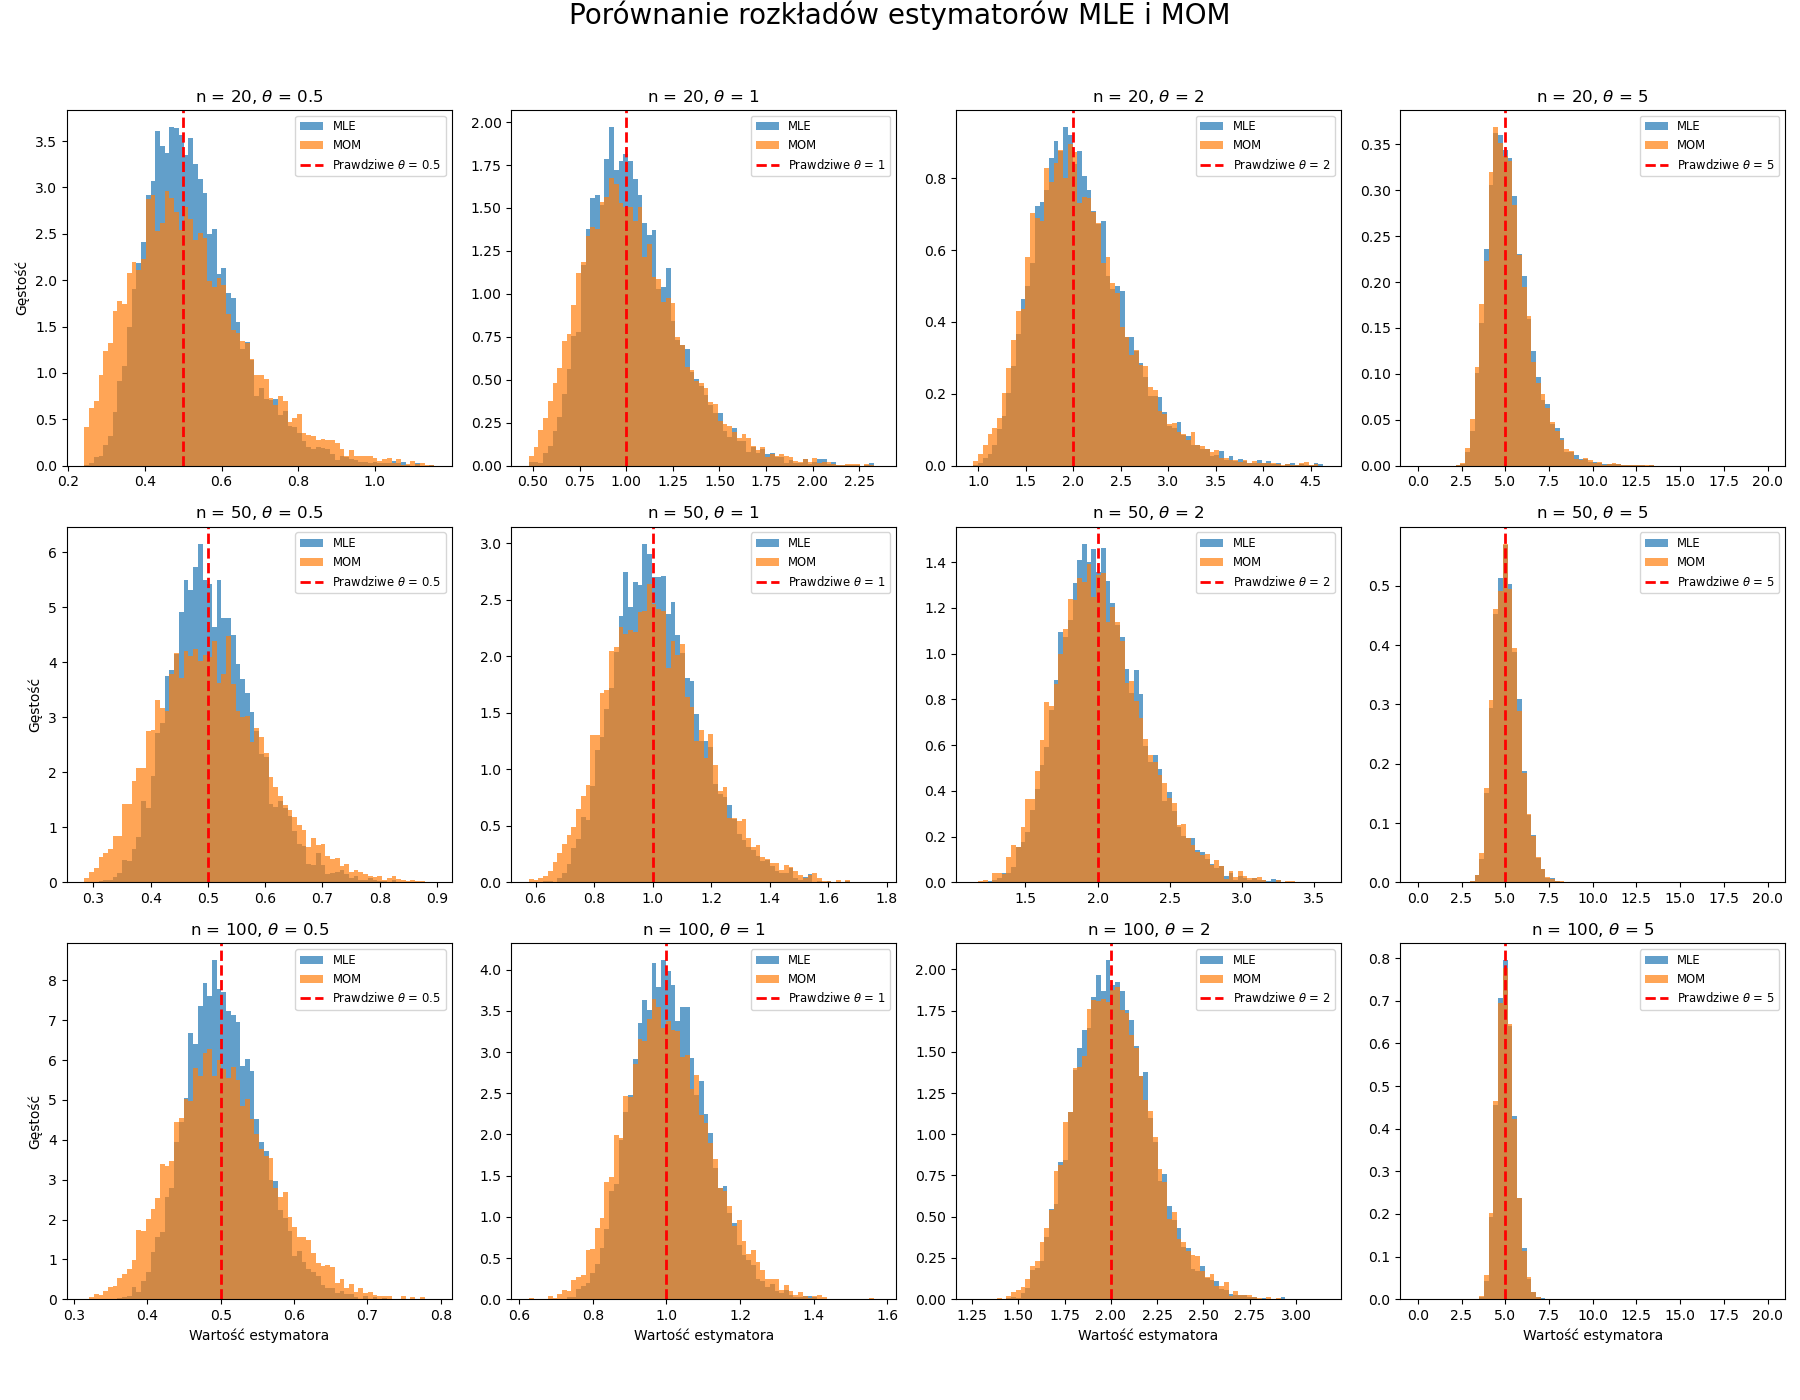
\includegraphics[width=0.9\textwidth]{../plots/zad4a/wykresy_rozkładow/histograms_mle_mom_comparison.png}
        \end{center}

        \begin{center} 
            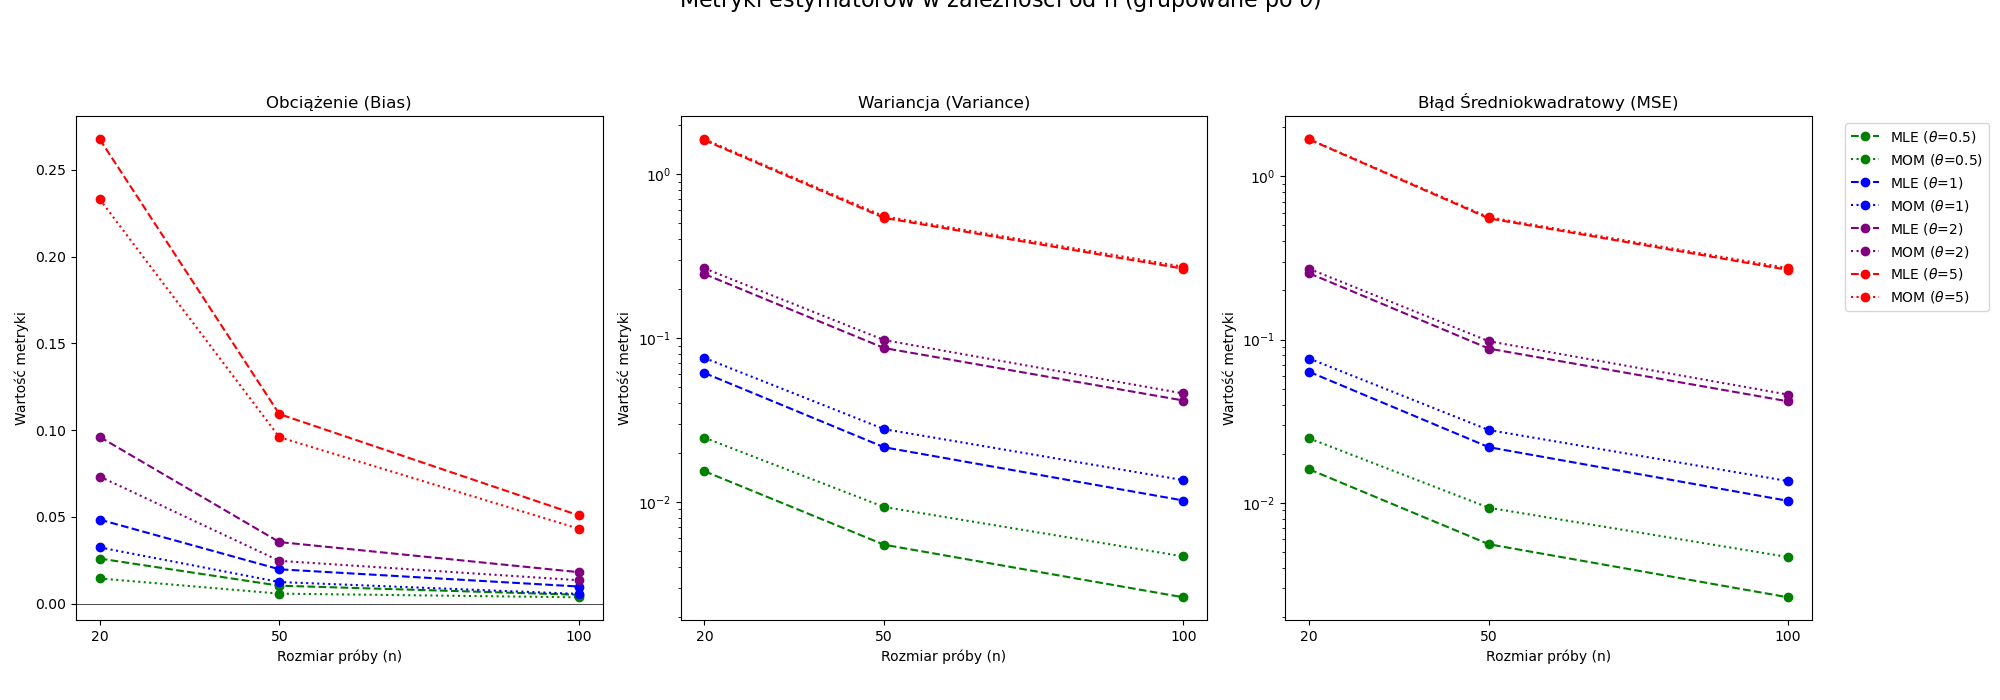
\includegraphics[width=0.9\textwidth]{../plots/zad4a/wykresy_metryk/metrics_vs_n.png}
        \end{center}

        \begin{center} 
            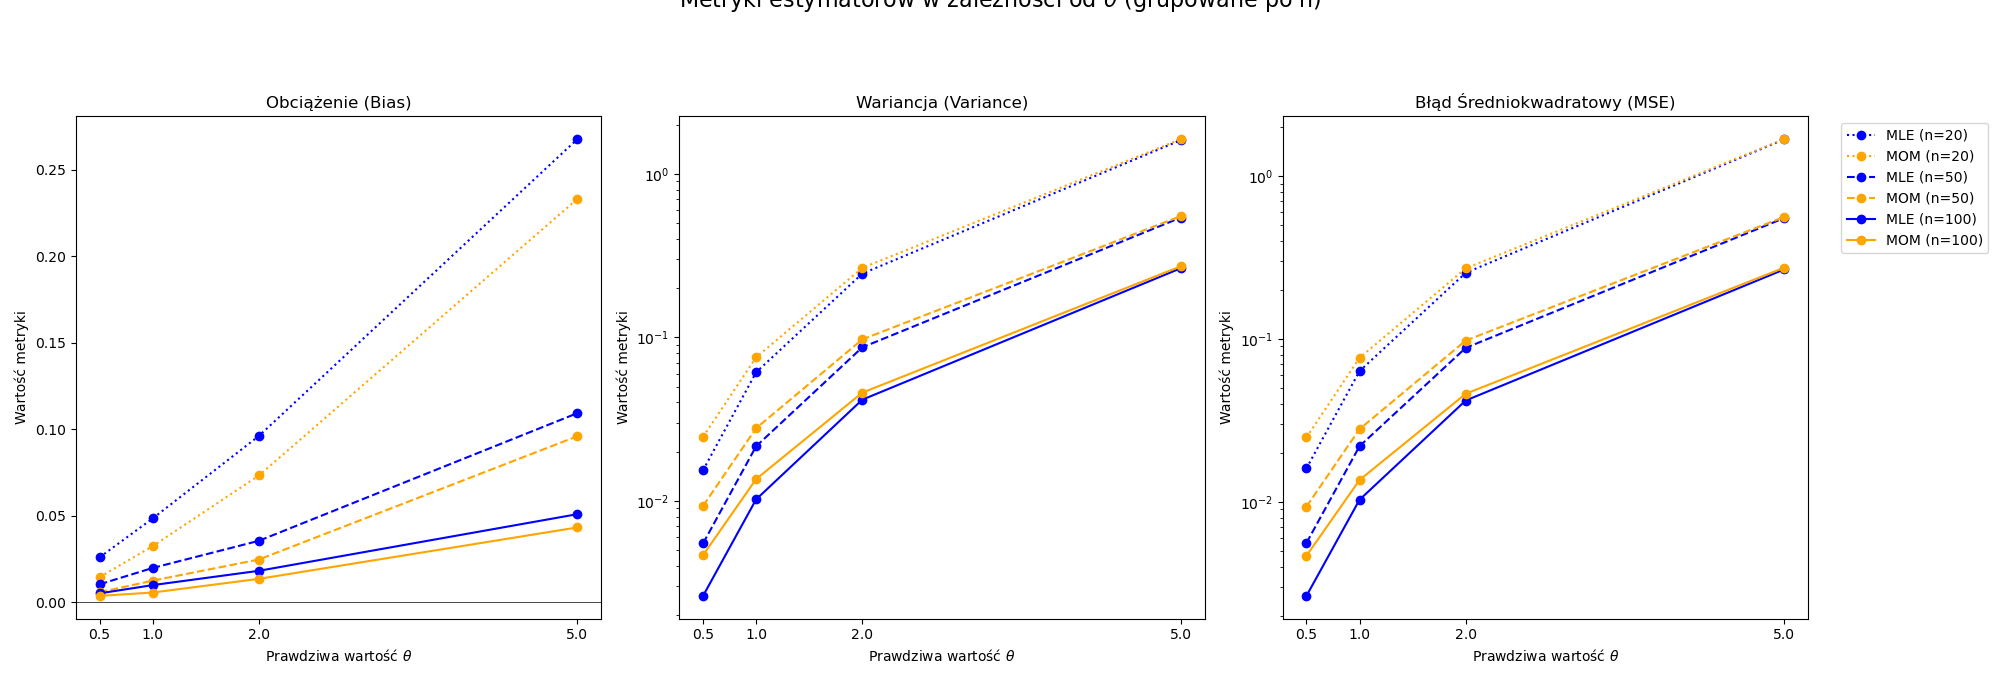
\includegraphics[width=0.9\textwidth]{../plots/zad4a/wykresy_metryk/metrics_vs_theta.png}
        \end{center}

    \begin{itemize}
        \item \textbf{Wariancja:} Dla wszystkich scenariuszy, rozkład $\hat{\theta}_{\text{MLE}}$ jest trochę bardziej skoncentrowany wokół prawdziwej wartości $\theta$ niż rozkład $\hat{\theta}_{\text{MOM}}$.
        \item \textbf{Obciążenie i Skośność MOM:} MLE ma trochę większy Bias niż MOM. 
    \end{itemize}

    Na przeprowadzonych eksperymetanch wydajsność obu esymatorów jest do siebie bardzo zbliżona. Im większy parametr $\theta$, 
    tym różnice między estymatorami są mniejsze, a obie sytamcje są coraz bardziej obciążone.

\newpage

\section{Zadanie 4b}

    W zadaniu przeprowadzono symulację w celu porównania właściwości estymatora $\hat{\theta}_{\text{MLE}}$ oraz estymatora $\hat{\theta}_{\text{MOM}}$
    dla parametru lokalizacji $\theta$ w rozkładzie $\text{Lognorm}(\theta, \sigma)$, gdy parametr $\sigma$ jest znany.

    \subsection{Definicje Estymatorów}

    \begin{itemize}
        \item \textbf{Estymator Największej Wiarogodności:} $\overline{\ln(X)}$ 
        \item \textbf{Estymator Metody Momentów:} $ \ln(\bar{X}) - \frac{\sigma^2}{2} $
        
    \end{itemize}

    \subsection{Analiza Estymatora}

        \begin{center}
            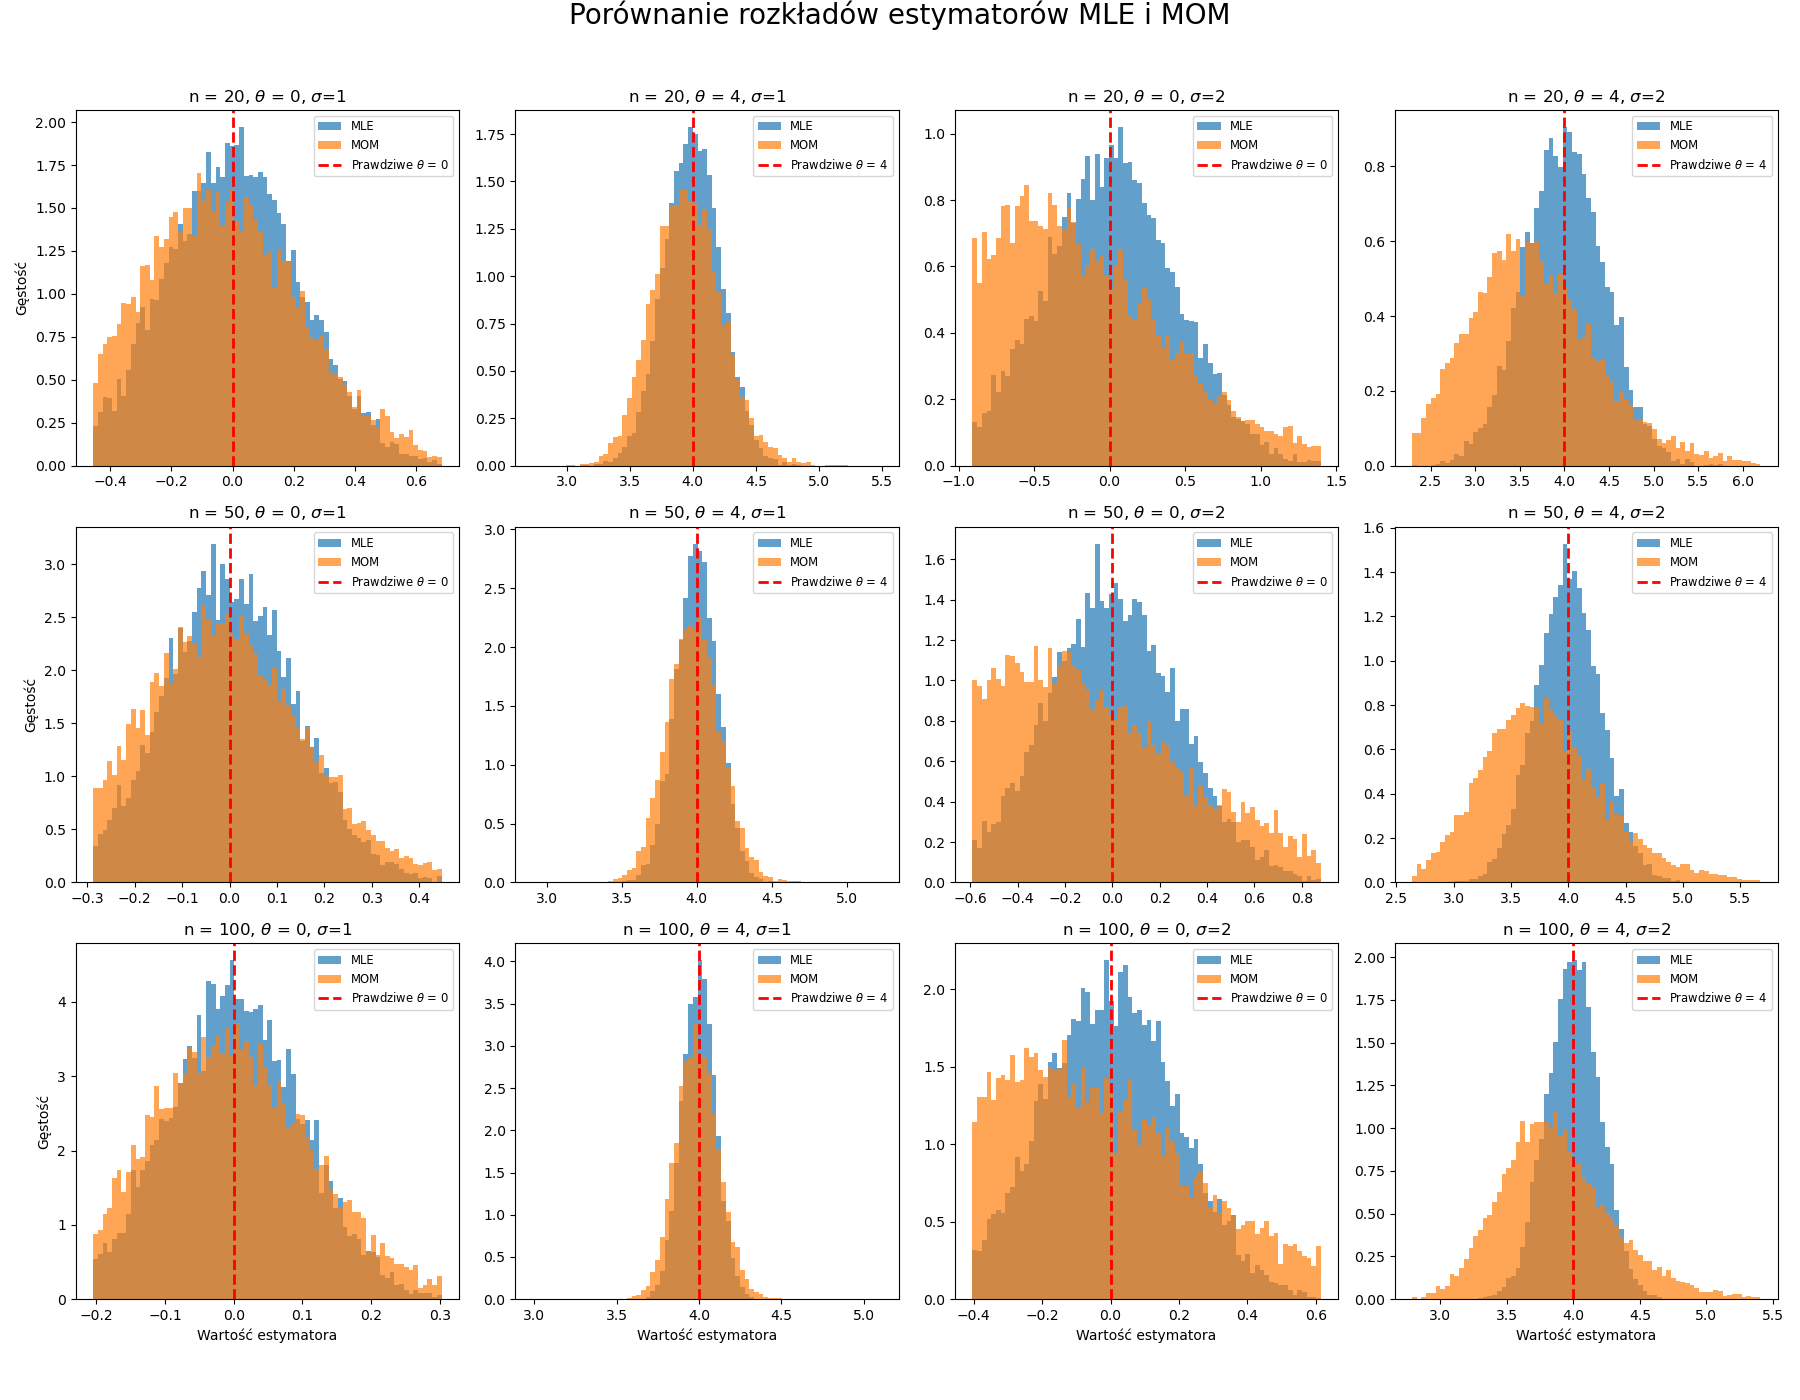
\includegraphics[width=0.9\textwidth]{../plots/zad4b/wykresy_rozkładow/histograms_mle_mom_comparison.png}
        \end{center}

        \begin{table}[h!]
            \centering
            \caption{Bias, Wariancja i MSE estymatorów}
            \label{tab:stats}

            \textbf{Bias} \\
            \csvautotabular{../plots/zad4b/statystyki_metryki/bias_table.csv}
            \vspace{0.5em}

            \textbf{Wariancja} \\
            \csvautotabular{../plots/zad4b/statystyki_metryki/variance_table.csv}
            \vspace{0.5em}

            \textbf{MSE} \\
            \csvautotabular{../plots/zad4b/statystyki_metryki/mse_table.csv}

        \end{table}

        \vspace{1em} % Dodatkowa przestrzeń po tabelach
    \subsubsection*{Wnioski z Porównania Estymatorów}

    Analiza wykresów oraz danych w tabelach metryk potwierdza, że estymator $\hat{\theta}_{\text{MLE}}$ jest estymatorem preferowanym dla parametru lokalizacji $\theta$ w rozkładzie lognormalnym, charakteryzując się znacznie lepszymi właściwościami statystycznymi.

    \begin{itemize}
        \item \textbf{Obciążenie (Bias):}
        Estymator $\hat{\theta}_{\text{MLE}}$ jest teoretycznie \textbf{nieobciążony} 
        i w symulacji jego Bias jest bliski zeru we wszystkich scenariuszach. Natomiast $\hat{\theta}_{\text{MOM}}$ jest 
        \textbf{zauważalnie mocno obciążony}, zwłaszcza dla małych prób ($n=20$) i dużych wartości parametru skali $\sigma$.
        
        \item \textbf{Wariancja i Precyzja:}
        $\hat{\theta}_{\text{MOM}}$ charakteryzuje się \textbf{sporą wariancją} w porównaniu do $\hat{\theta}_{\text{MLE}}$. 
        Rozkład $\hat{\theta}_{\text{MLE}}$ jest węższy i bardziej skupiony wokół prawdziwej wartości $\theta$, co czyni go estymatorem 
        \textbf{bardziej precyzyjnym} i \textbf{efektywnym}.
        Różnica w wariancji jest szczególnie wyraźna w scenariuszach z dużym $\sigma$ ($\sigma=2$).
        
        \item \textbf{Wpływ Parametrów $(\theta, \sigma)$:}
        Jakość estymacji jest \textbf{najgorsza} (najwyższe MSE i Wariancja) w scenariuszach z dużym parametrem skali ($\sigma=2$). 

        \item \textbf{Wpływ $n$:}
        Wraz ze wzrostem rozmiaru próby ($n=20 \to 100$), \textbf{MSE oraz Bias obu estymatorów maleją}.
        Jednak spadek MSE dla $\hat{\theta}_{\text{MOM}}$ jest wolniejszy, 
        co podkreśla jego gorszą efektywność w porównaniu do $\hat{\theta}_{\text{MLE}}$.
    \end{itemize}

    W przyadku tego rozkładu estymator MLE jest zdecydowanie lepszym wyborem niż estymator MOM.


\end{document}
